% intsup
%
\documentclass[10pt,dvips]{article}
%\documentclass[10pt,twocolumn,dvips]{article}
\usepackage[english]{babel}
\usepackage{epsfig}
%\usepackage{fancyheadings}
%\usepackage[T1]{fontenc}
%\usepackage[latin1]{inputenc}
%\usepackage{twocolumn}
%\usepackage{verbatim,moreverb,doublespace}
%\usepackage{rotate,lscape,dcolumn,array,rotating,latexsym}
%
%\input{epsf}
%
% for somebody (I forget now !)
%\textwidth 175mm
%\textheight 225mm
%\topmargin -4.5mm
%
% for somebody else (I also forget now !)
%\textwidth 6.6in 
%\textheight 239mm
%\topmargin -15mm
%\leftmargin -2.0in
%
% for (IEEE single-column format)
%\textwidth 6.875in
%\textheight 8.875in
%\topmargin -0.6in
%\oddsidemargin 0mm
%\evensidemargin 0mm
%
% for HPCA (IEEE two-column format)
%\textwidth 6.5in
%\textheight 8.875in
%\topmargin -0.4in
%\oddsidemargin 0mm
%\evensidemargin 0mm
%
% for ISPASS
\textwidth 6.5in
\textheight 8.875in
\topmargin -0.4in
\oddsidemargin 0mm
\evensidemargin 0mm
%
%
% turn the following (linespread) on to 1.6 for "double space"
%\linespread{1.6}
%
%
% some publishers want no page numbers for final print
%\pagestyle{empty}
%
\begin{document}
%
% turn this off when publishing for real (to recoup the space !)
%\parskip 1mm
%
%
\title{Supplemental Data for Characterization of Register
Temporal Locality}
%
%
\author{
D. Morano\\
Northeastern University\\
dmorano@ece.neu.edu\\
}
%
%
% some publishers do not want a data in the final print
\date{25th October 2002}
%
\maketitle
%
% uncomment the following for page with no page numbers (for IEEE)
%\thispagestyle{empty}
%
%
\begin{abstract}
%
This paper is a supplement to a paper submitted to ISPASS'03.
In that paper
various intervals associated with register and memory accesses
were explored.
This paper primarily provides additional data that was not
presented in that paper.
Detail about the three register access intervals for each of
the benchmark programs examined is presented.
Additionally, new data is presented for all of the benchmarks
on the read and write access frequencies for the registers 
by register address.
%
\end{abstract}
%
%
%\vspace{-0.25in}
\section{Introduction}
%\vspace{-0.15in}
%
This paper provides supplementary data on the access intervals
for registers and memory locations over what has been previously
reported in the paper \textit{Implications of Register and 
Memory Temporal Locality for
Distributed Microarchitectures} by Khalafi, et al ~\cite{khalafi_ispass03}.
In that paper, data for register access intervals was provided
in an abbreviated form.  In this paper, we present the data
again but separated out for each of the ten benchmark programs
that were investigated.  Further, we present additional data
about register read and write access frequencies per register
address that was not presented.
We only present new data for register access intervals.
A large set of data for the memory variable access intervals
was already provided in the preceding paper.

The rest of this paper is organized as follows.
In Section 2 provides an additional example to illustrate
how the various access intervals are calculated.
Section 3 presents our additional characterization results.
In Section 3 we discuss some of the data results.
Section 4 summarizes the present work.
%
%
%
%\vspace{-0.25in}
\section{Example Interval Calculation}
%\vspace{-0.15in}
%
A simple and contrived 
code example illustrating the meaning and method of calculation
of the three
intervals, that we have defined, is shown in Figure \ref{tab:code2}.
Unlike the previous example, this one features a loop.
%
\begin{table}
\begin{center}
\caption{{\em Simple code example illustrating the different types of
access intervals.}
Alongside the instructions are the particular events generated
from those instructions and any intervals that can be calculated
as a result.}
\label{tab:code2}
\vspace{+0.1in}
\begin{tabular}{l|l|l|l}
\hline 
label&instruction&event&intervals determined\\
\hline 
\hline 
I1&\verb"r1 <= c1"&def(r1)& \\
\hline
I2&\verb"r2 <= r1 + c2"&def(r2), use(r1)&
access-use(r1)=1, def-use(r1)=varies \\
\hline
I3&\verb"beq r2, I2"&use(r2)&
access-use(r2)=1, def-use(r2)=1 \\
\hline
I4&\verb"r1 <= c3"&def(r2)&
useful-lifetime(r1)=2001\\
\hline
\end{tabular}
\end{center}
\end{table}
%
In this simple code example, the terms \textit{c1} and \textit{c2} are
arbitrary
immediate constants encoded within the instructions.
We assume that this code loops 1000 times and then control falls
through the conditional branch at $ I3 $.  More precisely,
instructions $ I2 $ and $ I3 $ execute 1000 times each.
This snippet is interesting because it shows how the various
access intervals can sometimes vary widely in their average
behavior from each other when just simple code constructs are 
encountered.

For all three access intervals we are investigating, their statistics
are given in Table \ref{tab:stats} for this simple code example.
%
\begin{table}
\begin{center}
\caption{{\em Access Interval Statics on the 
Simple Code Example of Table 1.}
The mean and standard deviation is given for access-use, useful-lifetime,
and def-use intervals.}
\label{tab:stats}
\vspace{+0.1in}
\begin{tabular}{l|l|l}
\hline 
interval&mean&standard deviation\\
\hline 
\hline 
access-use&1.5&0.5\\
useful-lifetime&3.0&63.2\\
def-use&500.5&645.1\\
\hline
\end{tabular}
\end{center}
\end{table}
%
In particular, note the widely varying means for the useful-lifetime
(3.0) and the def-use (500.5) intervals.
As might be expected, the access-use interval is shorter (on average)
than the other two but it may be somewhat interesting to see the
difference between the other two interval averages.
In each case, the standard deviation gives a clue to the amount
of dispersal in the data.  Instruction $ I2 $ is the cause of the
def-use interval dispersal.
While the useful-lifetime of all registers (when averaged together)
is kept low due to the presence of the def in instruction $ I2 $
even the def in instruction $ I4 $ does not bring the useful-life
average over about 3.0.  In fact, without the def of instruction $ I4 $,
the average useful-lifetime of all registers would have stayed at
about 1.0 with a standard deviation of about 0.0.
The key feature of this code example is the use (by the compiler or
a human programmer) of setting up the invariant variable in register $ r1 $
prior to entering the loop.
Hopefully, this would occur commonly in optimizing compilers.
Of course, real code contains more interesting cases than shown
in this example but this illustrates how the various intervals
can vary from each other due to various code factors.

Not illustrated here but which occurs not uncommonly is that
writes to variables (whether registers or memory locations)
can be abandoned due to a change in control flow from a conditional
branch.  In these sorts of cases, the compiler may have setup some
variable expecting the control flow to proceed in a certain direction,
which is subsequently thwarted by the actual execution.
%
%
%\vspace{-0.25in}
\section{Characterization Results}
%\vspace{-0.15in}
%
Here we present data for both the three access intervals
presented previously but with the full set of data shown
for each benchmark program.
In addition to the access intervals, we also show register
read and write frequencies.  This data has not been previously
presented in any form.
%
%\vspace{-0.25in}
\subsection{Register Access Interval Results}
%\vspace{-0.15in}
%
In this section, we show the register access interval results for
our ten benchmark programs.
Unlike the previous paper, we show the data collected
for each program for individual benchmark programs 
rather than overlaid on a single graph.  
Data
for register access-use, useful-lifetime, and def-use intervals
are shown in turn.
%
% RRINT
%
The data for register access-use intervals are
shown in Figures \ref{fig:aa_rrint} 
and \ref{fig:ab_rrint}.
Results from benchmark programs BZIP2, COMPRESS, CRAFTY, GCC, and GO
are shown in Figure \ref{fig:aa_rrint} while the results
from programs GZIP, IJPEG, MCF, PARSER, and VORTEX are shown in
Figure \ref{fig:ab_rrint}.
%
\begin{figure}
\centering
\epsfig{file=aa_rrint.eps,width=6.0in}
\caption{{\em Register Access-Use Intervals.} 
Data results for the 
BZIP2, COMPRESS, CRAFTY, GCC, and GO programs are shown.
The density is shown on the left and the distribution is shown
on the right.
All intervals are measured in dynamic numbers of executed instructions.}
\label{fig:aa_rrint}
\end{figure}
%
\begin{figure}
\centering
\epsfig{file=ab_rrint.eps,width=6.0in}
\caption{{\em Register Access-Use Intervals.} 
Data results for the
GZIP, IJPEG, MCF, PARSER, and VORTEX programs are shown.
The density is shown on the left and the distribution is shown
on the right.
All intervals are measured in dynamic numbers of executed instructions.}
\label{fig:ab_rrint}
\end{figure}
%
%
% RLIFE

The data for register def-last-use (or useful-lifetime) intervals are
shown in Figures \ref{fig:aa_rlife} 
and \ref{fig:ab_rlife}.
%
\begin{figure}
\centering
\epsfig{file=aa_rlife.eps,width=6.0in}
\caption{{\em Register Def-Last-Use Intervals.} 
Data results for the 
BZIP2, COMPRESS, CRAFTY, GCC, and GO programs are shown.
The density is shown on the left and the distribution is shown
on the right.
All intervals are measured in dynamic numbers of executed instructions.}
\label{fig:aa_rlife}
\end{figure}
%
\begin{figure}
\centering
\epsfig{file=ab_rlife.eps,width=6.0in}
\caption{{\em Register Def-Last-Use Intervals.} 
Data results for the
GZIP, IJPEG, MCF, PARSER, and VORTEX programs are shown.
The density is shown on the left and the distribution is shown
on the right.
All intervals are measured in dynamic numbers of executed instructions.}
\label{fig:ab_rlife}
\end{figure}
%
%
% RUSE

The data for register def-use intervals are
shown in Figures \ref{fig:aa_ruse} 
and \ref{fig:ab_ruse}.
%
\begin{figure}
\centering
\epsfig{file=aa_ruse.eps,width=6.0in}
\caption{{\em Register Def-Use Intervals.} 
Data results for the 
BZIP2, COMPRESS, CRAFTY, GCC, and GO programs are shown.
The density is shown on the left and the distribution is shown
on the right.
All intervals are measured in dynamic numbers of executed instructions.}
\label{fig:aa_ruse}
\end{figure}
%
\begin{figure}
\centering
\epsfig{file=ab_ruse.eps,width=6.0in}
\caption{{\em Register Def-Use Intervals.} 
Data results for the
GZIP, IJPEG, MCF, PARSER, and VORTEX programs are shown.
The density is shown on the left and the distribution is shown
on the right.
All intervals are measured in dynamic numbers of executed instructions.}
\label{fig:ab_ruse}
\end{figure}
%
%

Figure \ref{fig:a_rover} shows (top to bottom)
the three types of access intervals:
access-use, useful-lifetime, and def-use.
For each type of access interval, the data for each of the
ten benchmark programs are overlaid on the same graph.
For each access interval type, both a density 
and a distribution is provided.
This presentation of the register interval access
data has been already presented but
is repeated here for the reader's convenience.
%
\begin{figure}[tb]
\centering
\epsfig{file=a_rover.eps,width=6.5in}
\caption{{\em Register Access Intervals.} 
Data results for all programs are shown overlaid.
The density is shown on the left and the distribution is shown
on the right.
All intervals are measured in dynamic numbers of executed instructions.}
\label{fig:a_rover}
\end{figure}
%
As can be seen from the graphs of Figure \ref{fig:a_rover},
all of the benchmark programs perform similarly and have
rather short (20 or less) interval lengths for most of each type
of access interval.
%
%
%

For better clarity,
in Figure \ref{fig:a_rcum} we show the cumulative 
register interval data over all
benchmark programs.  
That figure shows, in order, all three of the access
intervals that we explored: access-use, useful-lifetime, and def-use.
%
\begin{figure}[tb]
\centering
\epsfig{file=a_rcum.eps,width=6.0in}
\caption{{\em Cumulative Register Intervals over all benchmarks.} 
The density is shown on the left and the distribution is shown
on the right.
All intervals are measured in dynamic numbers of executed instructions.}
\label{fig:a_rcum}
\end{figure}
%
%
%\vspace{-0.25in}
\subsection{Register Access Frequency Results}
%\vspace{-0.15in}
%
In this section we show the frequencies for reads and writes
for each individual register.  Each register is identified by
its architected address.  Separate accounting was maintained for
reads and writes so the corresponding data is also separated.
%
% RRDWR

The data for register access frequencies verses register address are
shown in Figures \ref{fig:aa_rrdwr} 
and \ref{fig:ab_rrdwr}.
The frequencies for reads and writes are each normalized to 
all of the register reads and writes respectively.
This essentially is a density of register accesses with respect
to register address.
Results from benchmark programs BZIP2, COMPRESS, CRAFTY, GCC, and GO
are shown in Figure \ref{fig:aa_rrdwr} while the results
from programs GZIP, IJPEG, MCF, PARSER, and VORTEX are shown in
Figure \ref{fig:ab_rrdwr}.
%
\begin{figure}
\centering
\epsfig{file=aa_rrdwr.eps,width=6.0in}
\caption{{\em Register Read and Write Access Frequencies.} 
Data results for the 
BZIP2, COMPRESS, CRAFTY, GCC, and GO programs are shown.
The read frequencies are shown on the left and the write frequencies are
shown on the right.
All accesses are shown at specific register addresses.}
\label{fig:aa_rrdwr}
\end{figure}
%
\begin{figure}
\centering
\epsfig{file=ab_rrdwr.eps,width=6.0in}
\caption{{\em Register Read and Write Access Frequencies.} 
Data results for the
GZIP, IJPEG, MCF, PARSER, and VORTEX programs are shown.
The read frequencies are shown on the left and the write frequencies are
shown on the right.
All accesses are shown at specific register addresses.}
\label{fig:ab_rrdwr}
\end{figure}
%
%
Figures \ref{fig:cum_rread} and \ref{fig:cum_rwrite} show the cumulative
densities over
register addresses for register reads and register writes
respectively.  
On the MIPS ISA, registers $ r0 $ through $ r31 $ are integer registers.
Registers $ r64 $ through $ r85 $ are floating point registers.
Other registers (which do not get much use) are various status
or control registers (usually for floating pointer operations).
It should be noted that register $ r0 $ is hardwired to
the value zero and is a read-only register.
For reference, register $ r29 $ is the stack pointer.
Further, register $ r28 $ is the pointer to the global offset
table and is only written once at the start of the program.
The data shown is only for the execution of 500 million instructions
after skipping the first 100 million, so the single write of register
$ r28 $ would not show up in this data anyway.
Registers $ r26 $ and $ r27 $ are never written or read
by any of the benchmark programs investigated (the ten that we executed).
Finally, register $ r39 $ (visible in some of the graphs)
is actually the sum of all register
accesses for MIPS registers with address 39 or higher.
As a result, this is essentially the sum of all accesses to floating point
data or control/status registers.
%
\begin{figure}
\centering
\epsfig{file=cum_rread.eps,width=6.0in}
\caption{{\em Cumulative Register Read Frequencies.} 
The cumulative register read frequencies over all benchmark programs
are shown.
All accesses are shown at specific register addresses.}
\label{fig:cum_rread}
\end{figure}
%
\begin{figure}
\centering
\epsfig{file=cum_rwrite.eps,width=6.0in}
\caption{{\em Cumulative Register Write Frequencies.} 
The cumulative register write frequencies over all benchmark programs
are shown.
All accesses are shown at specific register addresses.}
\label{fig:cum_rwrite}
\end{figure}
%
%
%\vspace{-0.25in}
\section{Discussion}
%\vspace{-0.15in}
%
Examination of the various register access intervals for
each program shows rather similar behavior across most all
programs.
However, when examining the register access frequency data for
each program, shown in Figures \ref{fig:aa_rrdwr} and \ref{fig:ab_rrdwr},
it is evident that most programs make use of the architected registers
in noticeably different ways. 
Although allocation of architected registers is largely done by
the compiler (all programs were written in the C programming language),
some registers have special standardized meanings as mentioned
in the previous section.

While all programs make use of their memory stacks, typified by
reads and writes to register $ r29 $, some make much more use of it
than others.  The BZIP2 and IJPEG program make relatively low use
of their stack as compared with the others.  In contrast, the programs
CRAFTY, PARSER, and VORTEX make especially high use of their stacks.
Another difference among the programs is the way they make use of
register $ r0 $ (fixed in the MIPS ISA to the value zero).
The GZIP, MCF, PARSER, and VORTEX program make especially high
use of that while the others make more moderate or smaller use.
No programs write register $ r0 $ since it is fixed as read-only in the ISA.
Although all of the benchmark program investigates are "integer"
oriented programs, some make substantial use of the floating
point register anyway.  The COMPRESS, and IJPEG programs make
noticeable use of the floating point registers while the other programs
make either a small or entirely negligible use of them.
Interestingly, the COMPRESS program reads the 
floating point registers almost as much as it writes them, but 
this is not the case for the IJPEG program (more on this later).
In the case of IJPEG, it writes floating point register much more than
it reads them.  This generally indicates that conditional control flow is
abandoning writes that occur before conditional branches.
Although this contributes towards its register useful-lifetimes being
zero for these cases (reference Figure \ref{fig:ab_rlife}), 
the effect does not appear to be significant as compared with the
other benchmarks.

It is interesting to note generally that the register read frequencies
are quite similar for the GCC, GO, and MCF programs.
This is also the case for the CRAFTY, PARSER, and the VORTEX
programs.  The PARSER and VORTEX programs are especially
similar even though the purpose of each program is different
(PARSER performs word processing and word indexing 
while VORTEX is a database kernel).
For write frequencies, they appear to be 
largely more similar across the programs than was the case for read
frequencies.  The notable exceptions are CRAFTY, GZIP, PARSER, and 
VORTEX all having more register writes in the 8 to 13 range of
register address than the others.  GZIP also has a singularly large
percentage of write to register $ r1 $ than any of the others.

Another important feature of these graphs is that write frequencies
(for almost all programs) do not match the corresponding read
frequencies of the same program.  This behavior is especially
evident around the program memory stacks, which use architected register
$ r29 $.
However, most registers are written with different frequencies than
they are read.  
Although it is generally expected that one write to a particular
register might be read more than once, the case where more than one
write
to a register with only one or less succeeding read also occurs.
These cases are largely due to the register write being abandoned
due to intervening conditional control flow changes.
The different is register read and writes frequencies
is part of the reason why register useful-lifetimes
are normally so different from register def-use intervals.

If, for example, all registers were written and then followed by
one read before they were written again, then the register useful-lifetime
intervals and the register def-use intervals would be identical.
But this is generally not the case.  Rather, some registers are
written more often than read (giving rise to smaller average useful-lifetimes)
while the reverse can also occur (giving rise to average smaller def-use
intervals).
Further, even if the cumulative read and write frequencies were
the same in any given program, we still do not have information
on particular read and write instances (only that the average frequencies
are the same).  These and other effects generally make all three
types of register access intervals investigated to be different.
%
%
%
%
%\vspace{-0.25in}
\section{Summary}
%\vspace{-0.15in}
%
We have presented supplementary data on register access intervals
that was not presented in the previous paper.
Three types of intervals were explored.  There were:
access-use, useful-lifetime, and def-use intervals.
Additionally, we presented data for register read and write
access frequencies.

%
\bibliographystyle{latex8}
\bibliography{intsup}
%
\end{document}
%
%
%
